\chapter{PLOS CB Paper}
\label{chap:ploscb}

\section{Background}

DNA, the material basis of genetic information, is a flexible polymer comprising two strands of nucleotides that coil around each other, at a rate of 10.5 base pairs per turn.
When subjected to torsional stress, DNA can either writhe and form 3-dimensional loops, or twist around itself more or less tightly than in its relaxed state~\citep{travers2005}; both forms are referred to as DNA supercoiling, which is measured as the relative density of supercoils $\sigma$ compared to relaxed DNA.
DNA is positively supercoiled ($\sigma > 0$) when it is overwound, and negatively supercoiled ($\sigma < 0$) when it is underwound.
In bacteria, DNA is normally maintained in a moderately negatively supercoiled state, with a reference value of $\sigma=-0.06$ in \emph{Escherichia coli}~\citep{travers2005}.
DNA supercoiling plays an important role in the regulation of gene expression in bacteria~\citep{martisb.2019}, as it is highly dynamic, and varies in both space along the chromosome and time during the cell lifecycle~\citep{krogh2018}, and as the level of supercoiling at the promoter of a gene modulates the expression of that gene~\citep{forquet2021}.
Furthermore, gene transcription itself locally impacts the level of DNA supercoiling, resulting in an interplay between the supercoiling and transcription of neighboring genes~\citep{meyer2014}, which hints at a possible role for this coupling as an evolutionary force shaping genome organization~\citep{junier2016}.

\subsection{The Dynamic Nature of DNA Supercoiling}

The level of DNA supercoiling in bacteria is controlled by topoisomerases, enzymes that alter DNA supercoiling by cutting and rotating the DNA strands~\citep{duprey2021}; the two main topoisomerases being gyrase, which dissipates positive supercoiling by introducing negative supercoils at an ATP-dependent rate, and topoisomerase I, which oppositely relaxes negative supercoiling~\citep{martisb.2019}.
Many other processes however influence the level of DNA supercoiling.
According to the twin-domain of supercoiling~\citep{liu1987}, the transcription of a gene by RNA polymerase generates a buildup of positive supercoiling upstream of the gene, and negative supercoiling downstream of the gene, through the rotational drag that hampers the rotation of the polymerase around DNA.
At a larger scale, while the intrinsic flexibility of the DNA polymer would allow supercoils to propagate freely along its length, many nucleoid-associated proteins such as FIS, H-NS or HU bind to bacterial DNA (in addition to RNA polymerases), and create topological barriers that instead block the diffusion of supercoiling~\citep{travers2005}.
In bacteria, the level of DNA supercoiling can furthermore be affected by numerous environmental challenges.
Salt shock transiently increases negative DNA supercoiling in \emph{E. coli}~\citep{hsieh1991}; the acidic intracellular environment relaxes DNA in the facultative pathogen \emph{Salmonella enterica} var. Typhimurium~\citep{marshall2000}; and higher temperatures relax DNA in the plant pathogen \emph{Dickeya dadantii}~\citep{herault2014}.
These constraints overall result in a very dynamic DNA ``supercoiling landscape'' in \emph{E. coli}~\citep{visser2022}, with a supercoiling level that varies in both time during the bacterial lifecycle and space along the chromosome.
%, but increases negative supercoiling in the human pathogen \emph{Shigella flexneri}~\citep{tobe1995}. % Note: at the promoter of _virB_ yes, but not genome-wide

\subsection{DNA Supercoiling and Gene Regulation}

Many bacteria leverage the regulating effect of DNA supercoiling on gene transcription by modulating their DNA supercoiling level.
In several bacteria such as \emph{E. coli}, \emph{S. enterica}, or \emph{D. dadantii}, between 5\% and 15\% of genes were found to be sensitive to relaxation or hypercoiling of chromosomal DNA, with genes being up-regulated or down-regulated in each condition~\citep{peter2004, ferrandiz2010, webber2013, pineau2022a}.
DNA supercoiling might in particular be an especially important regulator of gene activity in bacteria with reduced genomes, such as the obligate aphid endosymbiotic bacterium \emph{Buchnera aphidicola}, which is nearly devoid of transcription factors~\citep{brinza2013}.

Moreover, selection can act on the level of DNA supercoiling in order to modulate the regulation of gene expression.
In 10 of the 12 populations in the Long-Term Evolution Experiment (LTEE), an increase in fitness was linked to mutations in the \emph{topA} and \emph{fis} genes, which participate in the regulation of the supercoiling level~\citep{crozat2010}.
When inserted into the ancestral strain, these mutations increased the level of negative supercoiling as well as the bacterial growth rate~\citep{crozat2005}, demonstrating that the level of DNA supercoiling can evolve as part of a regulatory response to new environments.

Finally, the regulation of gene expression by DNA supercoiling could be a force that participates in shaping the evolution of bacterial genomes themselves.
Indeed, supercoiling-sensitive genes tend to group in up or down-regulated clusters in \emph{E. coli}~\citep{peter2004}, \emph{S. enterica}~\citep{webber2013} and \emph{S. pneumoniae}~\citep{ferrandiz2010}, suggesting the possibility of an adaptive role in the co-localization of these clusters.
Indeed, synteny segments, or clusters of neighboring genes that show correlated expression patterns, are evolutionarily conserved across \emph{E. coli} and the distantly related \emph{Bacillus subtilis}~\citep{junier2016}, strengthening the hypothesis that these domains could play an important role in the regulation of bacterial gene expression.

\subsection{The Transcription-Supercoiling Coupling}

As we saw before, the process of transcribing a given gene generates an accumulation of positive supercoiling downstream of that gene, and of negative supercoiling upstream of that gene~\citep{liu1987}.
If a second gene is located closely enough to this first gene, the change in supercoiling at the promoter of the second gene will impact its transcription rate, as negative supercoiling usually facilitates promoter opening, and hence gene transcription~\citep{forquet2021}.
In turn, the second gene will also generate a change in supercoiling that affects the first gene, resulting in an interaction between the transcription levels of these two genes.
Depending on the relative orientation of these genes, several types of interactions are therefore possible: divergent genes reinforce their respective transcription level in a positive feedback loop, convergent genes inhibit the transcription of one another, and for tandem genes, the downstream gene up-regulates the upstream gene, while the upstream gene down-regulates the downstream gene.

This effect, which has been called the transcription-supercoiling coupling~\citep{meyer2014,sobetzko2016,elhoudaigui2019}, has been documented in several bacterial genetic systems.
In \emph{S. flexneri}, the \emph{virB} promoter is normally only active at high temperature, but can be activated at low temperature by the insertion of a phage promoter in divergent orientation~\citep{tobe1995}.
Similarly, the expression of the \emph{leu-500} promoter in \emph{S. enterica} can be increased or decreased by the insertion of upstream transcriptionally active promoters, depending on their orientation relative to \emph{leu-500}~\citep{elhanafi2000}.
The magnitude of this effect has also been explored in a synthetic construct that uses the inducible \emph{ilvY} and \emph{ilvC} \emph{E. coli} promoters, inserted on a plasmid in divergent orientations.
In this system, a decrease in the activity of \emph{ilvY} is associated with a decrease in \emph{ilvC} activity, and an increase in \emph{ilvY} activity with an increase in \emph{ilvC} activity as well~\citep{rhee1999}.

There are, however, hints that the biological relevance of the transcription-supercoiling coupling might not be confined to a few specific cases.
Indeed, in \emph{E. coli}, the typical size of topological domains, inside which the supercoiling generated by gene transcription can propagate, is usually around 10kb~\citep{postow2004}, and could reach up to 25kb~\citep{visser2022} in each direction.
As the average size of \emph{E. coli} genes is 1kb, and the average intergenic distance about 120bp~\citep{blattner1997}, this means that any single topological domain encompasses several genes that can potentially interact via the transcription-supercoiling coupling.
A statistical analysis of the relative position of neighboring genes on the \emph{E. coli} chromosome furthermore shows that genes that are up-regulated by negative supercoiling have more neighbors in divergent orientations, while genes that are down-regulated by negative supercoiling have more neighbors in converging orientations~\citep{sobetzko2016}, suggesting that the transcription-supercoiling coupling plays a role in regulating the activity of these genes.

\paragraph{}
In this article, we present a two-level individual-based model of gene expression at the whole-genome scale, in which gene transcription is regulated solely by DNA supercoiling, and in which populations of individuals evolve towards environment-specific gene expression targets through genomic rearrangements only.
Rather than attempting to give quantitative predictions of the  effect of the transcription-supercoiling coupling on the expression levels of genes in a given, static genetic system, our model aims at exploring the range of genomic organizations that can be generated by selection in order to regulate gene expression levels in different environments through the transcription-supercoiling coupling.
Using this model, we observe the emergence of complex environment-driven patterns of gene expression, and characterize the spatial organization of genes along the genome that underlie these patterns.
We first show that genes are locally organized in convergent or divergent pairs that leverage the transcription-supercoiling coupling to activate or inhibit one another.
Then, we show that this local organization is not entirely sufficient to fully account for the complex gene expression patterns that we observe, but that gene inhibition requires the interaction of a large number of genes.
Finally, we show that, in our model, genes form a dense genome-wide regulatory network, providing insight into the organization of bacterial genomes.


\section{An Evolutionary Model of the Transcription-Supercoiling Coupling}
\label{sec:ploscb:model}

\subsection{Individual-Level Model}
\label{sec:ploscb:indiv_model}

We define the genotype of an individual in our model as a single circular chromosome that is representative of a bacterial chromosome.
The chromosome consists in a fixed number of protein-coding genes, which are separated by non-coding intergenic segments of varying sizes, and has a basal supercoiling level $\sigma_{basal}$.
Each gene on the chromosome is characterized by its starting position (genes cannot overlap in our model), its orientation (on the forward strand or on the reverse strand), its length, and its basal expression level.
We define an environment by the shift $\delta\sigma_{env}$ that it imposes to the supercoiling level of the chromosome.
We then define the phenotype of an individual in a given environment as the gene expression levels that are solution of the system given by the interaction of its genes through the transcription-supercoiling coupling (described below), on a chromosome with a background supercoiling level of $\sigma_{basal} + \delta\sigma_{env}$.

\begin{figure}[H]
  \centering
  \begin{subfigure}[t]{0.44\textwidth}
    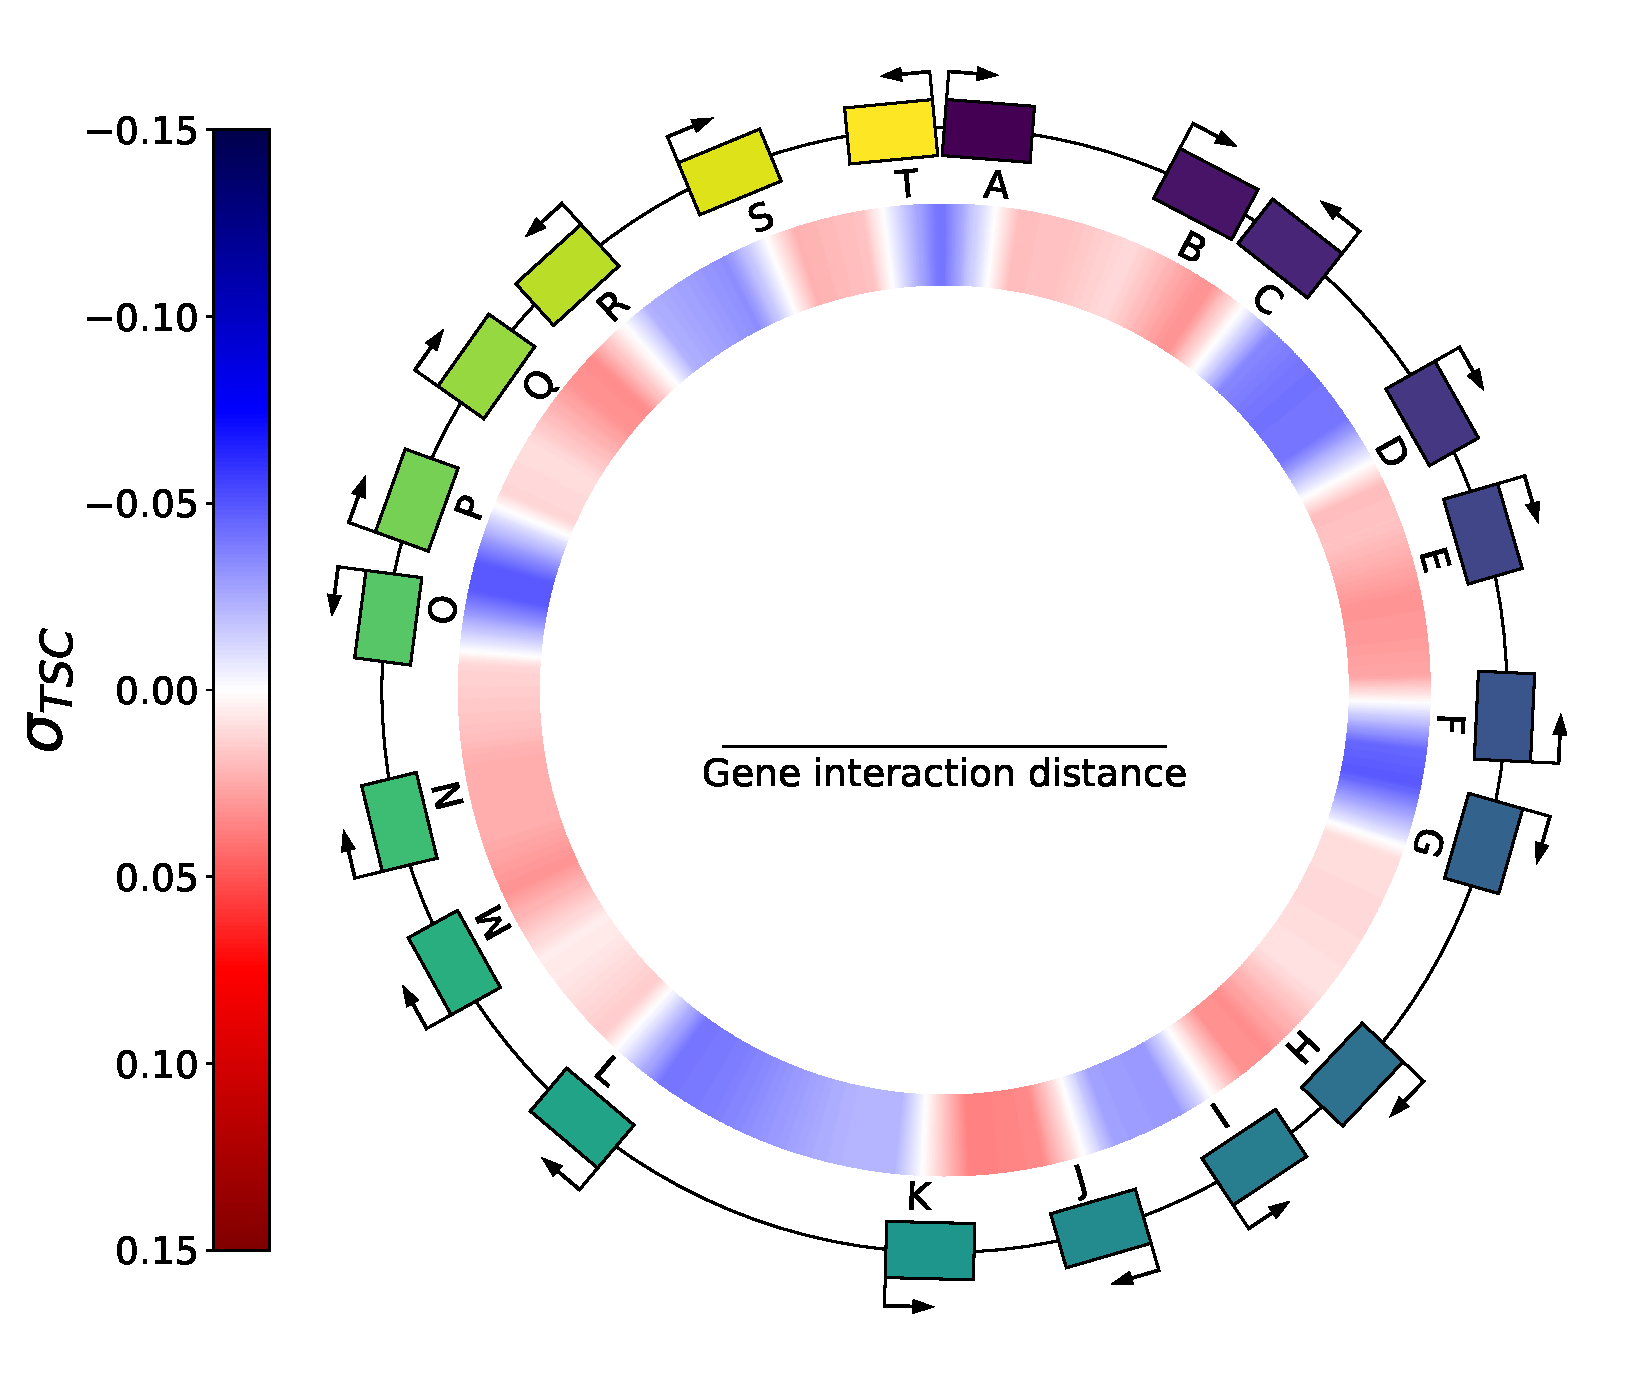
\includegraphics[width=\textwidth]{ploscb/img/random_genome_and_tsc.pdf}
    \label{subfig:ploscb:random_genome}
  \end{subfigure}
  \begin{subfigure}[t]{0.55\textwidth}
    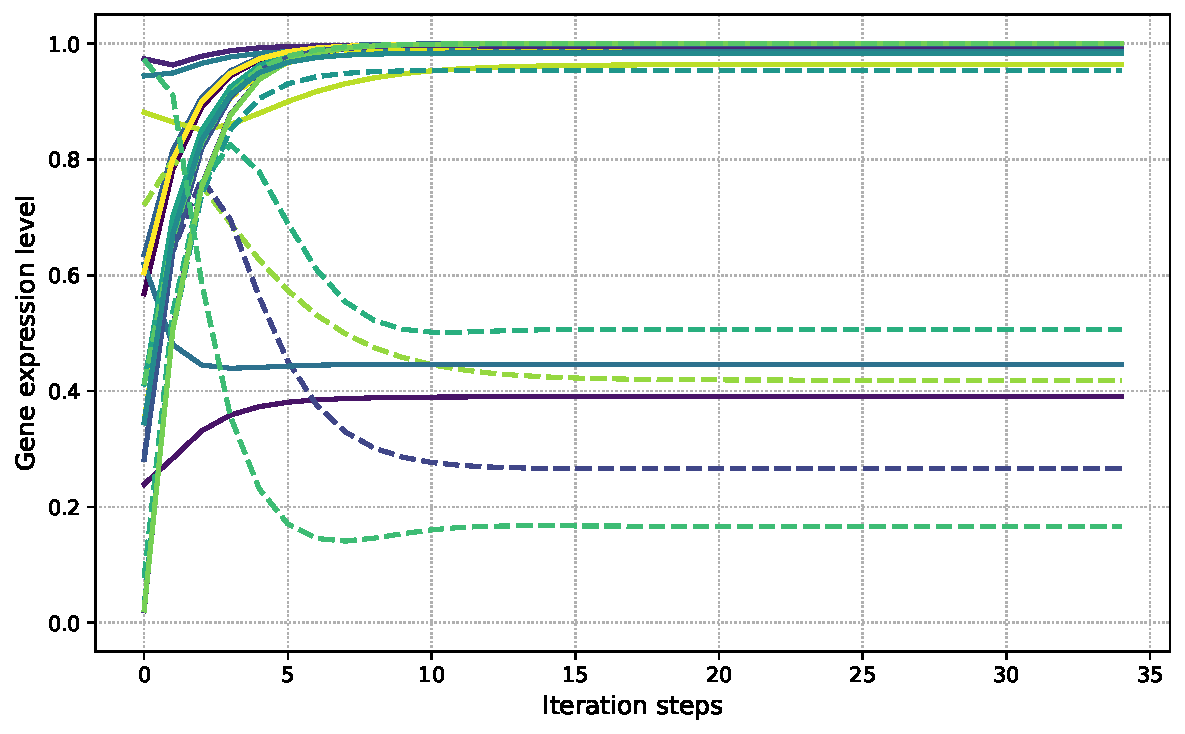
\includegraphics[width=\textwidth]{ploscb/img/random_gene_expr.pdf}
    \label{subfig:ploscb:random_expr}
  \end{subfigure}
  \caption[Example individual in the advanced model, evaluated in both environments]{Left: genome (outer ring) and level of supercoiling generated by transcription ($\sigma_{TSC}$, inner ring) of an example genome with 20 genes placed at random positions and orientations and colored by position, with a gene length and average intergenic distance of 1 kb each, and a basal supercoiling level of $\sigma_{basal} = -0.066$.
  The individual is evaluated in an environment in which $\delta\sigma_{env} = 0$.
  Right: evolution of the expression level of each gene of the individual during the computation of the solution to the system given by equations~\ref{eq:sigma},~\ref{eq:prom_energy}, and~\ref{eq:gene_activity}, starting from random initial values.
  Solid lines represent genes on the forward strand, dashed lines genes on the reverse strand, and gene colors are the same as on the genome.}
  \label{fig:ploscb:random_indiv}
\end{figure}

The genome of an example individual with 20 genes and a basal supercoiling $\sigma_{basal} = -0.066$ is shown on the left-hand side of Figure~\ref{fig:ploscb:random_indiv}.
Inside the genome is the resulting local level of DNA supercoiling when this individual is evaluated in an environment with a supercoiling shift of $\delta\sigma_{env}~=~0$.
As expected given the twin-domain model of supercoiling, we can observe a buildup in negative supercoiling (blue) between genes in divergent orientations, such as genes C and D or F and G, and a buildup in positive supercoiling (red) between genes in convergent orientations, such as genes J and K or Q and R.
The right-hand side panel of Figure~\ref{fig:ploscb:random_indiv} shows the computation of the stable state of gene expression levels for this individual.
Note that, in this model and throughout this article, we conflate
gene transcription rates with mRNA concentrations, as we assume that mRNAs degrade at a constant rate, and as transcription rates in our model are only affected by the effect of supercoiling on transcription.
We furthermore conflate transcription rates with expression levels, as we again assume proteins to be translated at a rate proportional to the associated mRNA concentrations and to degrade at a constant rate.

\paragraph{Effect of Transcription on Supercoiling}
For an individual with a genome containing $n$ genes, each expressed at a level $e_i$, we model the influence of the transcription of each gene on the level of supercoiling at the promoter of every other gene in the form of an $n$-by-$n$ interaction matrix.
The coefficient $\frac{\partial\sigma_i}{\partial e_j}$ at indices $(i, j)$ in this matrix represents the variation in DNA supercoiling at the promoter of gene $i$ due to the transcription of gene $j$.
The value of this coefficient is given by the following formula:

\begin{equation}
  \frac{\partial\sigma_{i}}{\partial e_j} = \eta \cdot c \cdot \max(1-\frac{d(i, j)}{d_{max}}, 0)
  \label{eq:dsigmade}
\end{equation}

$\eta$ represents the sign of the interaction, which depends on the position and orientation of gene $j$ relative to gene $i$, according to the twin-domain model.
If gene $j$ is upstream of gene $i$, and if it is on the same strand as (or points towards) gene $i$, then its transcription generates a buildup in positive supercoiling at gene $i$ ($\eta = 1$).
Conversely, if gene $j$ is upstream of gene $i$ but on the other strand than (or points away from) gene $i$, it generates a buildup in negative supercoiling at gene $i$ ($\eta = -1$).
If gene $j$ is instead located downstream of gene $i$, the sign of the interaction in each case is switched: $\eta = 1$ if the genes are on the same strand, and $\eta = -1$ otherwise.

We then apply a scaling coefficient $c$, which represents the intensity to which the transcription-generated torsion of DNA affects the local level of supercoiling.
Finally, the strength of the interaction decreases linearly with the distance $d(i, j)$ between the promoter of gene $i$, which is the position where the local level of supercoiling affects the probability that an RNA polymerase binds to the DNA and starts transcribing gene $i$, and the middle of gene $j$, which is the average location of the RNA polymerases that transcribe gene $j$, assuming that DNA is transcribed at a constant speed.
When this distance reaches a threshold of $d_{max}$, the two genes are considered to be too far away to interact and the effect vanishes.

\paragraph{Effect of Supercoiling on Transcription}
In order to compute the transcription level of a given gene, we first compute the opening free energy of its promoter, which depends on the local supercoiling level, following a sigmoidal curve that increases with negative supercoiling until a saturation threshold is reached~\citep{forquet2021}.
In order to model this effect, we adapted the equations and parameter values presented in~\cite{elhoudaigui2019}, which are based on the \emph{in vitro} analysis of the transcription of model bacterial promoters.
We first compute the local level of supercoiling $\sigma_i$ at the promoter of gene $i$, which is the sum of the background supercoiling level $\sigma_{basal} + \delta\sigma_{env}$ (which is constant along the genome for any given individual), and of the local variation in supercoiling caused by the transcription of every other gene (represented in Figure~\ref{fig:ploscb:random_indiv} as $\sigma_{TSC}$):

\begin{equation}
  \sigma_i = \sigma_{basal} + \delta\sigma_{env} + \sum_{j=1}^n\frac{\partial\sigma_{i}}{\partial e_j}e_j
  \label{eq:sigma}
\end{equation}

We compute the expression level of the gene using a thermodynamic model of transcription.
First, we compute the opening free energy $U_i$ of the promoter of gene $i$, which depends on $\sigma_i$, the level of supercoiling at the promoter and on $\sigma_0$, the level of supercoiling at which the opening free energy is at half its maximum level, according to the following sigmoidal function:

\begin{equation}
  U_i = \frac{1}{1 + e^{(\sigma_i - \sigma_0)/\epsilon}}
  \label{eq:prom_energy}
\end{equation}

The, we compute the expression level $e_i$ of gene $i$ using the promoter opening free energy, with a scaling constant $m$:

\begin{equation}
  e_i = e^{m (U_i - 1)}
  \label{eq:gene_activity}
\end{equation}

The transcription level of a gene is therefore expressed in arbitrary units between $e^{-m}$, the minimum expression level when the promoter is most hindered by supercoiling (when $U_i$ = 0), and 1, the maximum expression level, when the promoter is most activated by supercoiling (when $U_i$ = 1).
Throughout this manuscript, we will describe a gene as activated if its transcription level is above the mean of these two values $e_{1/2} = \frac{1}{2}(e^{-m} + 1)$, and inhibited otherwise.

\paragraph{Computation of Gene Expression Levels}

We define the phenotype of an individual in an environment (described by $\delta\sigma_{env}$) as the set of gene expression levels that is solution to the system given by equations~\ref{eq:sigma},~\ref{eq:prom_energy} and~\ref{eq:gene_activity}, in that environment.
In order to compute this phenotype, we numerically compute a solution to the system of equations using a fixed-point iteration algorithm, and starting from an initial state in which all genes are expressed at $e_{1/2}$.
A representative example of this computation can be found in Figure~\ref{fig:ploscb:random_indiv}: After an initially unstable phase, the algorithm quickly converges to a fixed point of expression levels.

\subsection{Evolutionary Model}
\label{sec:ploscb:evol_model}

Equipped with a model of the coupling between DNA supercoiling and gene transcription at the whole-genome scale, we now extend it into an evolutionary framework.
In order to study the transcriptional response of individuals placed in different environments, we model the evolution of a population of individuals, each behaving as described in subsection~\ref{sec:ploscb:indiv_model}, in two distinct environments named A and B.
Environment A is a DNA relaxation-inducing environment, with a supercoiling shift of $\delta\sigma_{env} = \delta\sigma_A > 0$, and environment B is a DNA hypercoiling-inducing environment, with a supercoiling shift of $\delta\sigma_{env} = \delta\sigma_B < 0$.
We then define three classes of genes with environment-specific target expression levels: \emph{AB} genes should be expressed in both environments, akin to housekeeping genes; \emph{A} genes should be expressed in environment A but not in environment B; and, conversely, \emph{B} genes should be expressed in environment B but not in environment A; both classes represent environment-specific genes such as the pathogenic genes of \emph{S. enterica} or \emph{D. dadantii}~\citep{cameron2012,herault2014}.

\paragraph{Fitness}
Let $(e^A_A, e^A_B, e^A_{AB})$ be the average gene expression level per gene type of an individual with $n$ genes in environment A, $(e^B_A, e^B_B, e^B_{AB})$ the average gene expression per type in environment B, and $(\tilde{e}^A_A, \tilde{e}^A_B, \tilde{e}^A_{AB})$ and $(\tilde{e}^B_A, \tilde{e}^B_B, \tilde{e}^B_{AB})$ be target expression values for each gene type in each environment.
For environment A, we choose to set $\tilde{e}^A_A = \tilde{e}^A_{AB} = 1$, and $\tilde{e}^A_B = e^{-m}$, which are respectively the maximal and minimal attainable gene expression levels in the model.
Similarly, for environment B, we set $\tilde{e}^B_B = \tilde{e}^B_{AB} = 1$, and $\tilde{e}^B_A = e^{-m}$.
We then compute the sum $g$ of the squared error between the mean and targeted expression levels for each gene type in each environment:

\begin{equation}
  g = \sum_{i\in\{A, B, AB\}}\left(e^A_i - \tilde{e}^A_i\right)^2 + \sum_{i\in\{A, B, AB\}}\left(e^B_i - \tilde{e}^B_i\right)^2
  \label{eq:gap}
\end{equation}

Finally, we define the fitness of the individual as $f = \exp(-k \cdot g)$, where $k$ is a scaling factor representing the intensity of selection: as $k$ increases, the difference in fitness, and hence in reproductive success, between individuals with different values of $g$ also increases.

\paragraph{Generational Evolutionary Algorithm}
At each generation, we compute the fitness of each individual, by computing their gene transcription levels in each environment, as previously described.
In order to create the next generation, we choose a parent from the current population for each individual in the new population, with a probability proportional to the fitness of the parent.
Then, we create the genome of the new individual by stochastically applying mutations to the genome of its parent.

\paragraph{Mutational Operator: Genomic Inversions}
As this work aims at studying genome organization, we chose to use genomic inversions as the only mutational operator, so that genes can be reordered on the chromosome through evolutionary time; note that other genomic rearrangements, such as translocations, can be modeled as a series of well-chosen consecutive inversions, and are therefore implicitly present in our model.

In order to perform a genomic inversion, we choose a start point and an end point uniformly at random, in the non-coding intergenic sections.
This ensures that genes cannot be broken apart by inversions, as we assume that gene losses are lethal and therefore never conserved.
Having chosen the ends of the inversion, we extract the DNA segment between these ends and insert it in the reverse orientation.
The inversion therefore switches the orientation of every gene inside the segment, but conserves the relative positions and distances of these genes.
Note that, contrary to the intergenic sections that are inside of the inversion, the intergenic sections that are at its boundaries change according to the position of the start and end points of the inversion, allowing the distances between genes to change over evolutionary time.

When mutating an individual, we first draw a number of inversions to perform from a Poisson law of parameter $\lambda = 2$, meaning that the offspring of the individual will on average undergo two inversions, and then perform each inversion in succession to obtain the final mutated offspring.


\section{Results}

In this section, we first show that, as in the proof-of-concept model presented in~\citep{grohens2021}, populations of individuals in the model presented in Section~\ref{sec:ploscb:model} evolve gene expression levels that match their targets in each environment.
Then, we show that, consistently with the theoretical expectations of the twin-domain model, the genomes of evolved individuals are enriched in pairs of divergent or convergent genes that leverage the transcription-supercoiling coupling to regulate gene expression.
Finally, we show that the gene regulatory network generated by the transcription-supercoiling coupling cannot simply be recapitulated by these local interactions, but rather encompasses the whole genome.

\subsection{Experimental Setup}

We evolved 30 populations of 100 individuals, each starting from clones of a random individual with 60 genes (20 of each type), for 1,000,000 generations.
The parameter values that we used are given in Table~\ref{tab:param_values}, and can be broadly grouped into genome-level parameters (gene length, intergenic distance, basal supercoiling level and supercoiling transmission distance) and promoter-level parameters (promoter opening threshold and energy, crossover width).
Both the genome-level parameters that describe the chromosome and the promoter-level parameters used to compute the transcriptional response to supercoiling were taken from experimental values measured in \emph{E. coli}.
In our model, we introduced the torsional drag coefficient as a new parameter that represents the influence of torsional drag on the local level of supercoiling, and empirically chose its value so that this effect is of the same magnitude as that of the other sources of supercoiling variations.

\begin{table}[H]
  \begin{center}
    \begin{tabular}{ l  l  r  c }
    \toprule
    \textbf{Parameter} & \textbf{Symbol} & \textbf{Value} & \textbf{Reference} \\
    \midrule
    %Population size & $N$ & 100 & \\
    %Number of genes & $n$ & 60 \\
    Gene length & $l$ & 1,000 bp & \cite{blattner1997} \\
    Initial intergenic distance & $d_0$ & 125 bp & \cite{blattner1997} \\
    Supercoiling transmission distance & $d_{max}$ & 5,000 bp & \cite{klein2021} \\
    Basal supercoiling level & $\sigma_{basal}$ & -0.066 & \cite{crozat2005} \\
    \midrule
    Torsional drag coefficient & $c$ & 0.03 & \\
    \midrule
    Promoter opening threshold & $\sigma_{opt}$ & -0.042 & \cite{elhoudaigui2019} \\
    Inverse promoter opening energy & $m$ & 2.5 & \cite{elhoudaigui2019} \\
    Crossover width & $\epsilon$ & 0.005 & \cite{elhoudaigui2019} \\
    \bottomrule
    \end{tabular}
    \end{center}
  \caption[Table of parameter values used for the advanced \emph{EvoTSC} runs]{Table of parameter values used in the evolutionary runs.
  The upper set of parameters is the genome-level parameters, the lower set the promoter-level parameters, both taken from the \emph{E. coli} literature; the middle parameter is a new addition from our model.}
  \label{tab:param_values}
\end{table}

The simulation was implemented in Python, with computationally heavy parts optimized using the \texttt{numba} package~\citep{lam2015}. The source code for the simulation, as well as the data analysis code, are available online at \url{https://gitlab.inria.fr/tgrohens/evotsc}.
Running the complete simulation took around 36 hours of computation on a server using a 24-core Intel Xeon E5-2620 v3 @ 2.40GHz CPU, with each replicate running on a single core and using approximately 300 MB of RAM.

\subsection{Evolution of Regulation by the Transcription-Supercoiling Coupling}

% Evolution works
\begin{figure}[H]
  \centering
  \hspace{-1.2cm}
  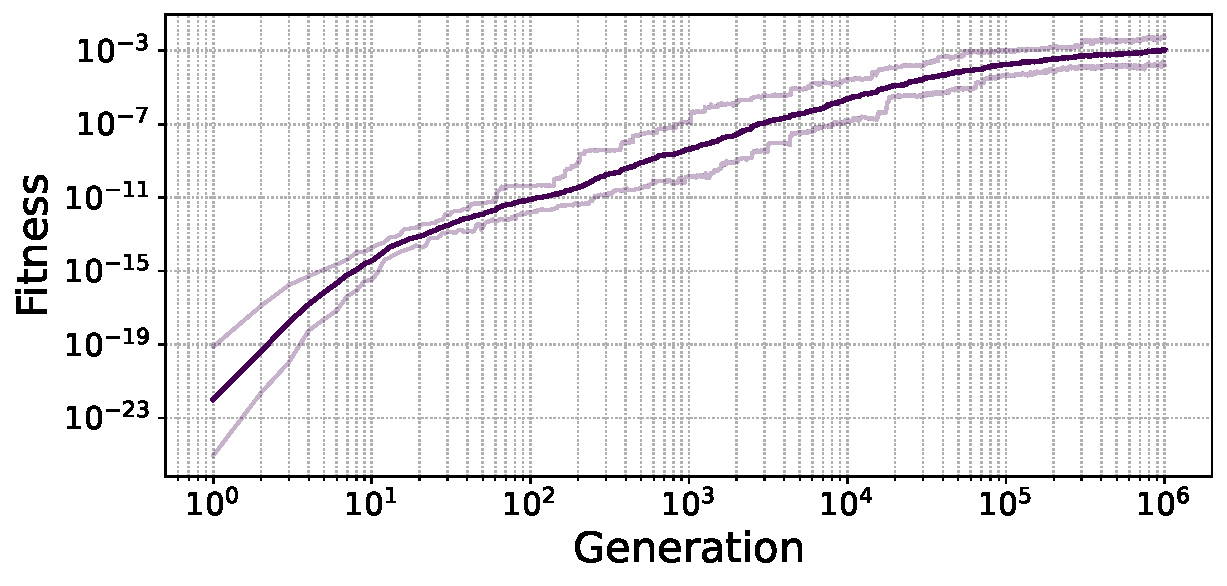
\includegraphics[width=0.75\textwidth]{ploscb/img/all_fitness.pdf}
  \caption[Average fitness during evolution in the advanced model]{Geometric average of the fitness of the best individual in each of the 30 replicates, at every generation.
  Lighter lines represent the first and last decile of the data.}
  \label{fig:ploscb:main_fitness}
\end{figure}

In our simulations, the fitness of the best individual in each population increases over evolutionary time, as shown in Figure~\ref{fig:ploscb:main_fitness}, meaning that evolution is able to select phenotypes that are closer and closer to the target. More precisely, the expression levels of the genes of each type in individuals in our model therefore evolve towards their respective targets, as previously defined in Section~\ref{sec:ploscb:evol_model}.

% Example genome in both environments
\begin{figure}[H]
  \centering
  \begin{elasticrow}[width=\textwidth]
  \elasticfigure{ploscb/img/genome_and_tsc_rep21_env_A.pdf}
  \elasticfigure{ploscb/img/genome_and_tsc_rep21_env_B.pdf}
  \end{elasticrow}
  \caption[Best individual at the end of evolution in one of the replicates in the advanced model, in both environments]{Genome of the best individual at the last generation of replicate 21, evaluated in environments A (left) and B (right).
  In addition to Figure~\ref{fig:ploscb:random_indiv}, the outer ring shows the state of each gene: dark color, activated -- light color, inhibited.
  The inner ring shows the level of transcription-generated DNA supercoiling at every position on the genome: Shades of blue represent negative supercoiling, and shades of red positive supercoiling.}
  \label{fig:ploscb:genomes}
\end{figure}

The genome of an example evolved individual at the end of the simulation is depicted in Figure~\ref{fig:ploscb:genomes}, along with its level of local supercoiling and gene activity in each environment.
Different activation patterns for each gene class are clearly visible on the genome of this individual.
Indeed, all \emph{AB} genes except one are activated (dark blue) in each environment, whereas 19 out of 20 \emph{B} genes are correctly inhibited (light green) in environment A (left) and 18 correctly activated (dark green) in environment B (right).
Conversely, 16 \emph{A} genes are activated (dark red) in environment A, and 16 inhibited (light red) in environment B.

The transcription-generated supercoiling represented in the inner ring furthermore changes consistently with the gene activation patterns between the two environments: red zones, where DNA is positively supercoiled, contain inhibited genes, whereas blue zones, where DNA is negatively supercoiled, contain activated genes.
This individual therefore shows that it is possible for evolution to adjust the gene expression levels of an individual in our model to an environment-dependent target, by relying only on the transcription-supercoiling coupling and on the relative positions of genes on the genome.

% Evolution of gene _activation_ by gene class
\begin{figure}[H]
  \begin{elasticrow}[width=\textwidth]
    \elasticfigure{ploscb/img/gene_activity_env_A.pdf}
    \elasticfigure{ploscb/img/gene_activity_env_B.pdf}
  \end{elasticrow}
  \caption[Average number of activated genes during evolution in the advanced model]{Average number of activated genes (with an expression level above $e_{1/2}$) of each type, out of 20, in the best individual at every generation, averaged over the 30 replicates, in environments A (left) and B (right).
  Lighter lines represent the first and last decile of the data.}
  \label{fig:ploscb:gene_activity_by_env}
\end{figure}

\paragraph{Evolution of Class-Specific Gene Expression Levels}
These results are however not specific to this particular individual.
Figure~\ref{fig:ploscb:gene_activity_by_env} shows that, averaging over all replicates, the number of activated genes in each class evolves towards their respective target.
In each environment, the average number of activated \emph{AB} genes quickly reaches nearly 20, its maximum value, as expected from their target; \emph{B} genes follow the same behavior, evolving towards nearly full activation in environment B and nearly full inhibition in environment A.
\emph{A} genes follow a slightly different course, as the number of activated \emph{A} genes seems to converge to approximatively 15 out of the expected 20 in environment A, but continues to decrease towards the expected 0 in environment B by the end of the simulations.

The incomplete match to their target of \emph{A} genes does however not come as a complete surprise.
Environment A is indeed characterized by a positive supercoiling shift $\delta\sigma_A > 0$, while environment B is characterized by a negative supercoiling shift $\delta\sigma_B < 0$.
As positive supercoiling hinders promoter opening, it is more difficult for a gene to have a high transcription rate in environment A than in environment B.
\emph{A} genes must therefore complete the more difficult task of being activated in the ``hard'' environment A, while being inhibited in the ``easy'' environment B.
Differentiated expression levels nonetheless evolve in our model for each type of gene, as a result of the different supercoiling levels imposed by the environmental conditions.

% Final message: evolution of hypercoiling-activated phenotype
\begin{figure}[H]
  \centering
  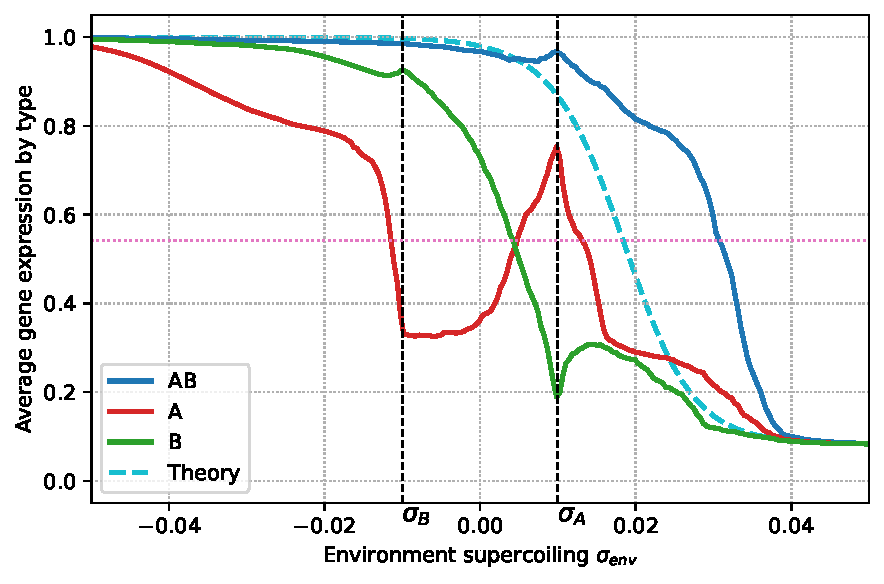
\includegraphics[width=\textwidth]{ploscb/img/activity_sigmas_avg.pdf}
  \caption[Average gene expression as a function of background supercoiling at the end of evolution in the advanced model]{Average gene expression level for each class of gene (\emph{A}, \emph{B}, and \emph{AB}), as a function of the background supercoiling level $\sigma_{basal} + \delta\sigma_{env}$, averaged over the best individual of each of the 30 replicates.
  The dash-dotted light blue line represents the average expression level of genes on a random genome, and the dashed light blue line represents the expression level of a single neighbor-less gene.
  The black vertical lines represent environments A and B, in which individuals evolve during the simulation, and the pink horizontal line marks $e_{1/2}$, the threshold above which a gene is considered active.}
  \label{fig:ploscb:activity_by_sigma}
\end{figure}

\paragraph{Evolution of Relaxation-Activated Genes}
In our model, the expression level of a gene increases exponentially with the opening free energy of its promoter, which itself increases as a sigmoidal function of negative supercoiling.
When measuring the response of an individual's genes to variation in the background supercoiling $\sigma_{basal} + \delta\sigma_{env}$, one could therefore expect a qualitatively similar response.

Figure~\ref{fig:ploscb:activity_by_sigma} shows the responses of genes of different types to the background supercoiling level (as explained in equation~\ref{eq:sigma}), and highlights striking differences between the expression of evolved, random, or isolated genes, as well as between the different gene types in evolved genomes.
The light blue lines in the figure serve as a reference point, showing the response of an isolated, non-interacting gene to environmental supercoiling (dashed line), and the average response (dash-dotted line) of genes on 30 random genomes, generated using the parameters from Table~\ref{tab:param_values}.
While \emph{AB} and \emph{B} genes (blue and green curves) display an expression level that decreases with the level of negative supercoiling, and that remains qualitatively similar to the behavior of random genes (dash-dotted line), \emph{A} genes display a completely different behavior.
These genes show a non-monotonic response to environmental supercoiling, as their expression level decreases until a local minimum in expression at $\delta\sigma_B$, then increases again even though negative supercoiling decreases until a local maximum at $\delta\sigma_A$, before decreasing again like the other kinds of genes.
In other words, \emph{A} genes present a phenotype of activation by environmental relaxation of DNA, for values between $\delta\sigma_B$ and $\delta\sigma_A$, even though the promoter activity of an isolated \emph{A} gene decreases with DNA relaxation.

The transcription-supercoiling coupling therefore provides a regulatory layer that mediates the transcriptional response to the global variation in DNA supercoiling caused by different environments.
Indeed, it remarkably allows in our model for the evolution of a response that is opposite not only to the response displayed by a non-interacting, neighborless gene, but also to the response of genes placed at random on a similar genome, demonstrating the importance of the relative position of genes on the genome.


\subsection{Evolution of Local Genome Organization}

Having characterized the different patterns of gene transcription that evolved in our simulations in response to the two different environmental conditions, we sought to determine the genome organization that necessarily underlies these patterns, since the only difference between individuals in our model is the relative position and orientation of the genes on their genome.

We started by studying genome organization at the local level, and measured the relative abundance of pairs of neighboring genes in every relative orientation: convergent, divergent, or in tandem.
The relative orientation between neighboring genes determines the mode of interaction between these genes, by applying the twin-domain model of transcription-generated supercoiling to the promoter of each gene: mutual activation for divergent genes, mutual inhibition for convergent genes, and activation (resp. inhibition) of the upstream (resp. downstream) gene by the downstream (resp. upstream) gene.

As the different gene types must evolve different activation patterns in each environment to have a high fitness in the model, we separated the pair counts by the type of each gene in the pair, resulting in 9 kinds of pairs.
Finally, in order to quantify the actual strength of the coupling between the genes in a given type of pair, we summed the total level of positive and negative supercoiling generated by the transcription of each gene in the pair at the promoter of the other gene for all relative orientations.
The results are presented in Figure~\ref{fig:ploscb:pair_results}, with the left-hand side panel showing the number of pairs of each kind, and the right-hand side panel the corresponding transcription-generated supercoiling levels.
Several patterns markedly emerge from the data.

\begin{figure}[H]
	\centering
	\begin{elasticrow}[width=\linewidth, sep=1em]
		\elasticfigure{ploscb/img/gene_pair_counts.pdf}
		\elasticfigure{ploscb/img/pos_neg_supercoiling_pairs.pdf}
	\end{elasticrow}
  \caption[Number of gene pairs and supercoiling effect per type of gene pair]{Interactions between pairs of neighboring genes.
  The left-hand side panel shows the number of pairs of each kind, split by the type of the first gene (sub-row) and of the second gene (sub-column) in the pair, and by relative orientation (bars in each sub-panel: convergent, divergent, upstream, or downstream).
  %As there are 20 genes of each type, and each gene appears in two pairs, the total number of pairs in each sub-row and sub-column is always 40.
  For instance, the top-right panel shows the influence of AB genes on B genes, and the bottom-left panel the influence of B genes on AB genes (in the same pairs).
  In that case, there are on average 7.8 \emph{AB} genes directly upstream of a \emph{B} gene (in red), or 7.8 \emph{B} genes directly downstream of an \emph{AB} gene (in green) on an evolved genome.
  % Talk about induced supercoiling?
  The right-hand side panel shows, for each kind of pair, the total amount of positive (red) and negative (green) transcription-generated supercoiling due to each gene type (sub-row) measured at the promoter of each gene type (sub-column), summing over all orientations, but in each environment.
  All data is averaged over the best individual of each of the 30 replicates, and box plots indicate the median and dispersion between the replicates.}
  \label{fig:ploscb:pair_results}
\end{figure}

% Divergent pairs: AB
\paragraph{Genomes Are Enriched in Divergent \emph{AB}/\emph{AB} Gene Pairs}
The most frequently found kind of gene pair in the evolved genomes is divergently oriented \emph{AB}/\emph{AB} pairs.
13 such pairs are found on average (see the \emph{AB}/\emph{AB} sub-panel on the left-hand side of Figure~\ref{fig:ploscb:pair_results}), out of a possible maximum of 20 (since any given gene can only be part of a single divergent pair), meaning that two-thirds of \emph{AB} genes are part of a divergent pair with another \emph{AB} gene.
The mostly divergent \emph{AB}\emph{AB} gene pairs generate an average negative supercoiling of around -0.012 at their promoters, in both environments (summing the positive and negative bars in the \emph{AB}/\emph{AB} sub-panel on the right-hand side of Figure~\ref{fig:ploscb:pair_results}).
This value is comparable in magnitude to but has the opposite sign than the shift in supercoiling caused by environment A ($\delta\sigma_A = 0.01$), showing that the interaction between neighboring genes can locally counteract the global shift in supercoiling caused by this environment in order to maintain high gene expression levels.

% Divergent pairs: A/A and B/B too, but not A/B
Genomes also contain divergent \emph{A}/\emph{A} and \emph{B}/\emph{B} gene pairs, although less frequently than divergent \emph{AB}/\emph{AB} pairs.
As both \emph{A} genes and \emph{B} genes must be conditionally expressed or inhibited depending on the environment, the unconditionally positive feedback loop resulting from a divergent orientation seems less evolutionarily favorable for \emph{A}/\emph{A} or \emph{B}/\emph{B} pairs than for \emph{AB}/\emph{AB} pairs.
Divergent \emph{A}/\emph{A} and \emph{B}/\emph{B} pairs moreover result in slightly weaker interactions (middle and bottom-right sub-panel of the right-hand side of Figure~\ref{fig:ploscb:pair_results}), in the environment in which these genes are active.
On the contrary, divergent \emph{A}/\emph{B} gene pairs are almost never found, and this is consistent with theoretical expectation, since \emph{A} and \emph{B} genes must no be expressed in the same environment.

The local organization of the genome in divergent \emph{AB}/\emph{AB} gene pairs therefore seems to be favored by evolution, as this pattern allows for a high expression of these genes in both environments, while divergent \emph{A}/\emph{B} gene pairs, which would lead to a lower fitness, are oppositely very rarely found in evolved genomes.

% Convergent pairs: A and B, mostly
\paragraph{Genomes are Enriched in Convergent \emph{A}/\emph{B} Gene Pairs}
The pattern in which \emph{B} genes appear most frequently, and \emph{A} genes very frequently (just after divergent \emph{A}/\emph{A} pairs), is in convergent \emph{A}/\emph{B} gene pairs.
In this case, each gene in the pair should theoretically inhibit the expression of the other gene.
In environment A, \emph{A} genes indeed generate an average positive supercoiling variation of 0.01 at the promoter of convergently oriented \emph{B} genes (the effect of \emph{B} genes on convergent \emph{A} genes in environment B is similar), decreasing their expression with a strength that is again comparable to the environmental change in supercoiling, whiles B genes are mostly inhibited and therefore do not impact \emph{A} genes.
In environment B, it is instead \emph{B} genes that strongly inhibit \emph{A} genes through the generation of positive supercoiling.

Convergently oriented \emph{A}/\emph{B} gene pairs therefore form toggle switches, or bistable gene regulatory circuits, in which the expression of one gene represses the expression of the other gene~\citep{gardner2000}.
In accordance with the targeted expression patterns of \emph{A} and \emph{B} genes, we therefore observe that the local organization of the genome into toggle switches, like the divergent \emph{A}/\emph{B} pairs, is favored by evolution in order to produce environment-dependent differentiated expression levels.


\subsection{Local Interactions Do Not Recapitulate the Regulatory Network}

In order to understand the extent to which the gene regulatory network generated by the transcription-supercoiling coupling can be reduced to the local organization into pairs of genes described above, we expanded our scope to study the behavior of subnetworks of neighboring genes of increasing sizes.

\begin{figure}[H]
  \centering
  %\begin{subfigure}[t]{\textwidth}
    %\centering
    %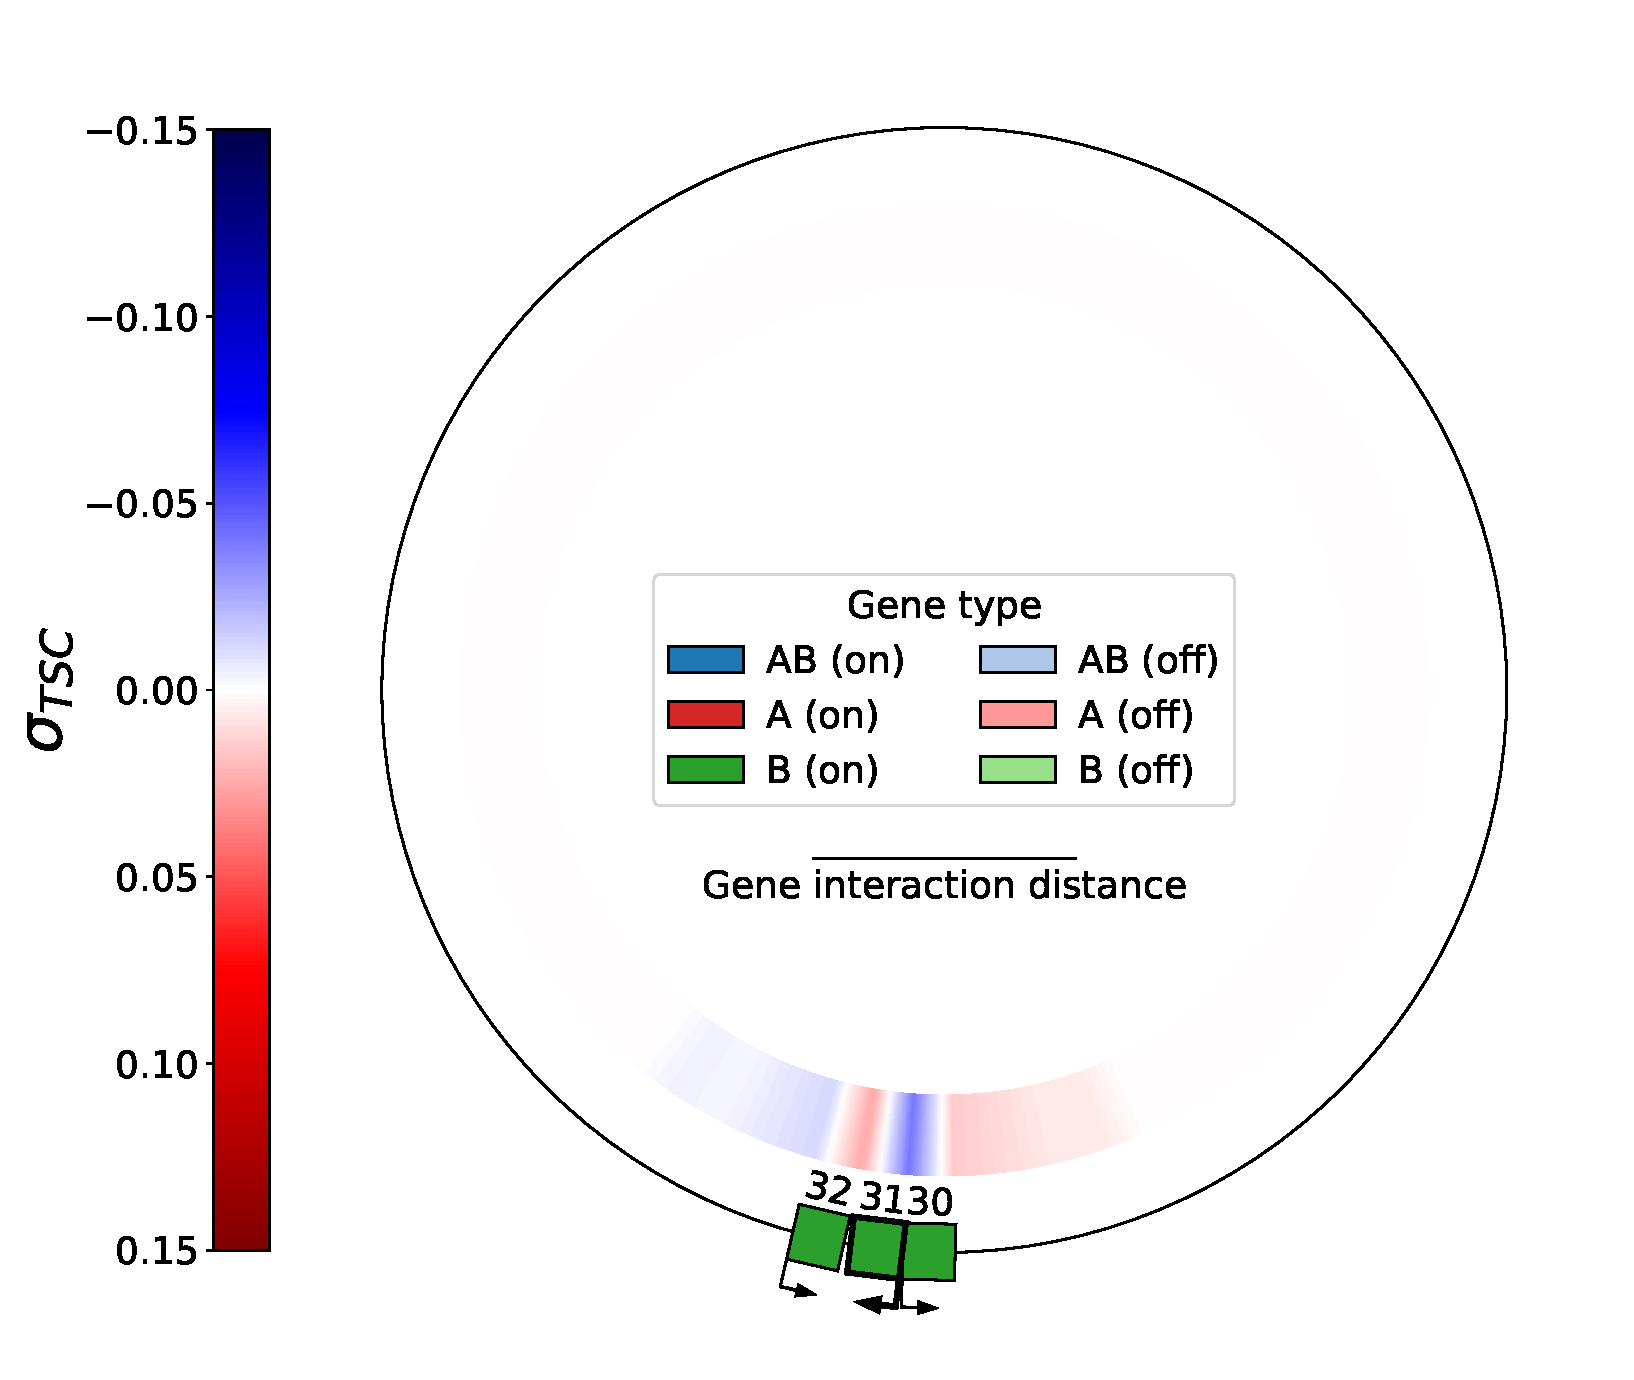
\includegraphics[height=7cm]{ploscb/img/sub_3_genes_30_env_A.pdf}
    %\hspace{-0.5cm}
    %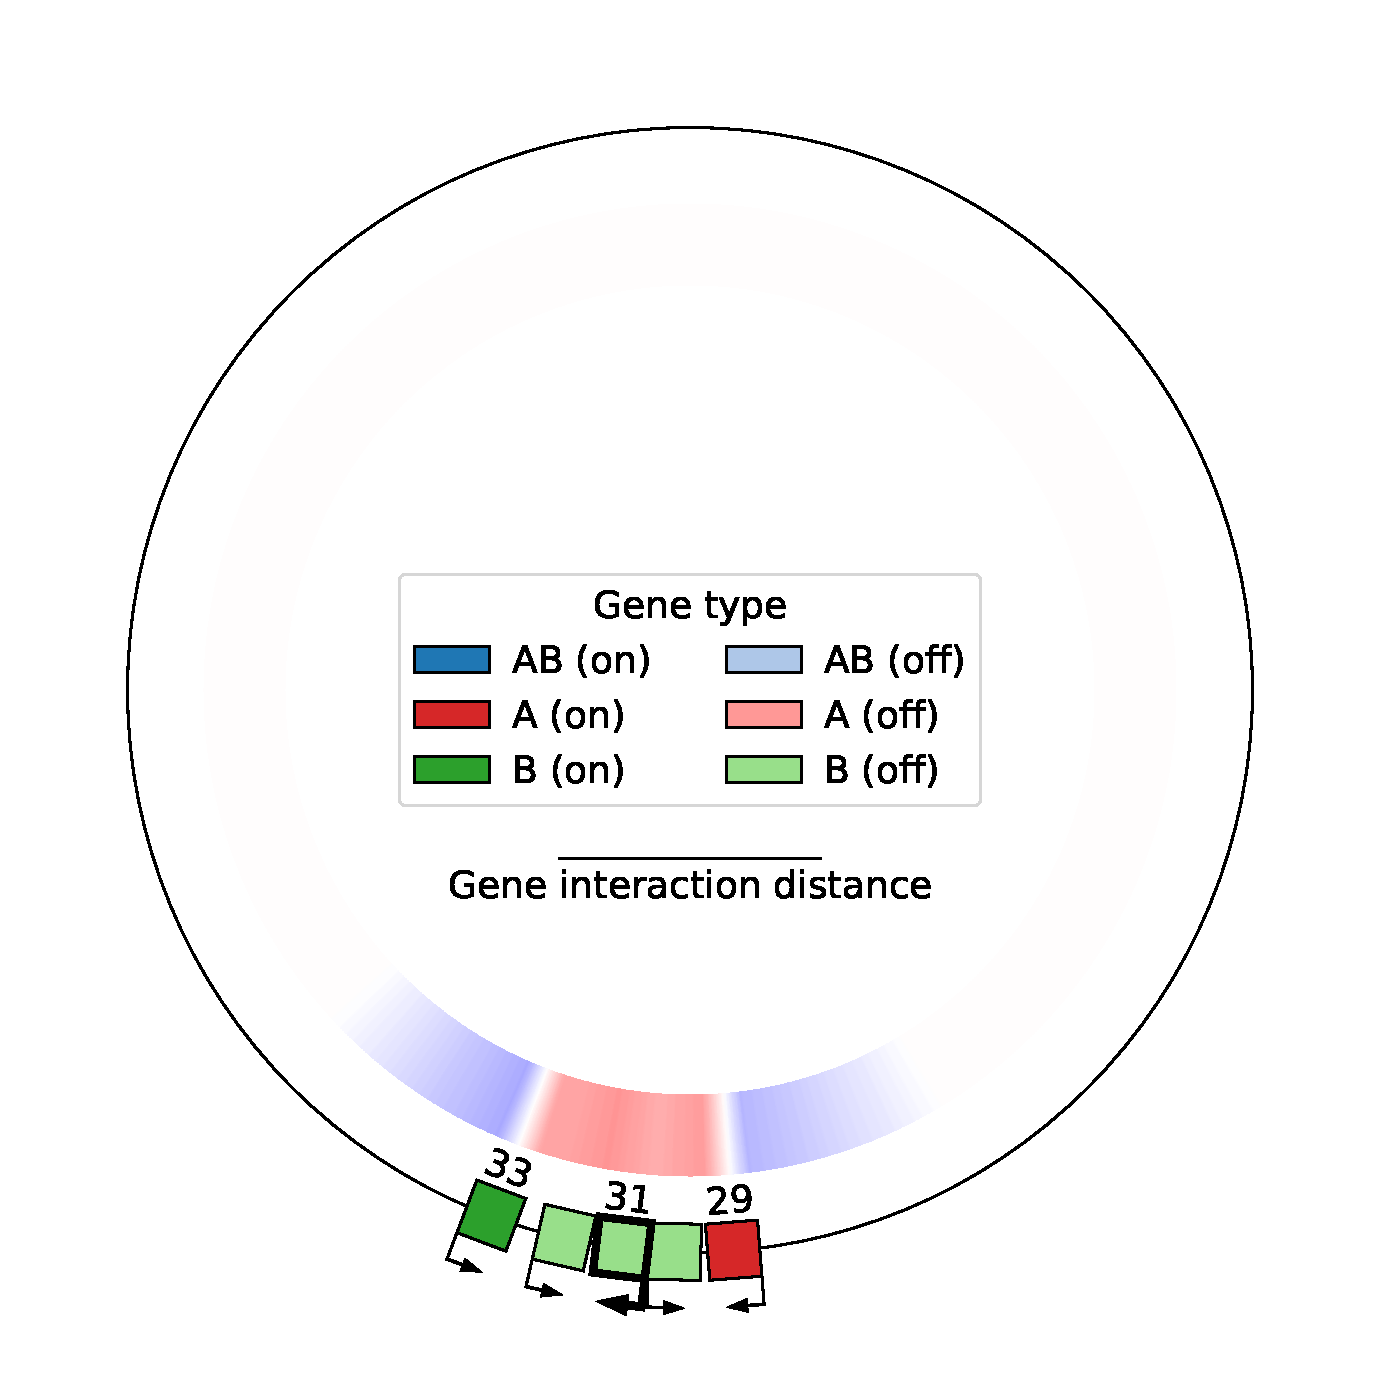
\includegraphics[height=7cm]{ploscb/img/sub_5_genes_29_env_A.pdf}
  %\end{subfigure}
  \begin{elasticrow}[width=\linewidth]
		\elasticfigure{ploscb/img/sub_3_genes_30_env_A.pdf}
		\elasticfigure{ploscb/img/sub_5_genes_29_env_A.pdf}
	\end{elasticrow}
  \begin{elasticrow}[width=\linewidth]
		\elasticfigure{ploscb/img/sub_7_genes_03_env_B.pdf}
		\elasticfigure{ploscb/img/sub_9_genes_02_env_B.pdf}
	\end{elasticrow}
  \caption[Example minimal subnetworks needed for gene inhibition in an evolved individual]{Top: subnetworks of size 3 (left) and 5 (right) centered around gene 31 (of type \emph{B}, in bold) of the best individual at the end of replicate 21, evaluated in environment A.
  Bottom: subnetworks of size 7 (left) and 9 (right), centered around gene 6 (of type \emph{A}, in bold) of the same individual, evaluated in environment B.
  }
  \label{fig:ploscb:subnetwork_examples}
\end{figure}

For every odd subnetwork size $k$ between 1 and the genome size, and for every gene on the genome, we extracted the subnetwork of size $k$ centered around that gene, and computed the expression level of every gene in the subnetwork, in the same way as for a complete genome, in each environment.
This allowed us to compute the minimum subnetwork size at which a gene has the same activation state as in the complete genome, which we interpret as an indicator of the complexity of the interaction network necessary to produce the activation state of that gene in the complete genome.
Two representative examples are presented in Figure~\ref{fig:ploscb:subnetwork_examples}, and the complete results are then shown in Figure~\ref{fig:ploscb:min_subnetwork}.

Figure~\ref{fig:ploscb:subnetwork_examples} depicts the subnetworks that are needed in order to obtain the inhibition of a representative gene of type \emph{A} in environment B, and of a representative gene of type \emph{B} in environment A, taken from the genome of an evolved individual.
The \emph{B} gene is not inhibited by a subnetwork of size 3, but needs a subnetwork of size 5 to be inhibited, and similarly, the \emph{A} gene is not inhibited by a subnetwork of size 7, but needs a subnetwork of size 9 to be inhibited.
In each case, increasing the size of the subnetwork by two (one gene on each side) completely changes the resulting gene expression levels, alongside with the associated level of transcription-generated supercoiling.
Indeed, in the top example, all 3 genes in the small subnetwork switch states when evaluated inside the larger subnetwork, and in the bottom example, the two \emph{B} genes and two out of the three central \emph{A} genes switch activation states when moving from the small to the large subnetwork.
In these examples, the activity of a gene is therefore not only dependent on its closest neighbors, but on a quite larger section of the genome.

\begin{figure}[H]
  \centering
  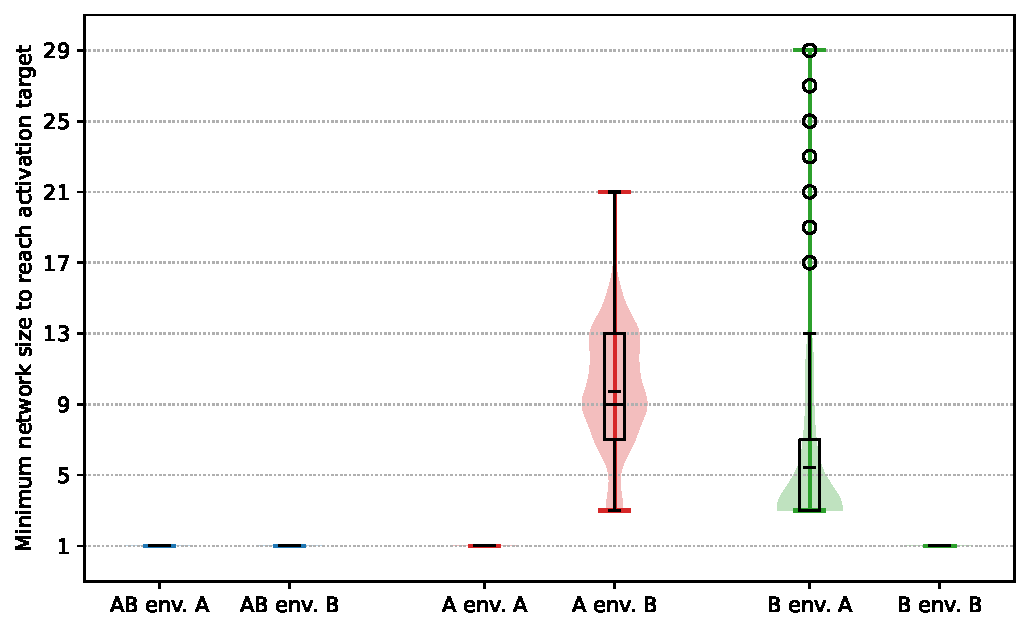
\includegraphics[width=\textwidth]{ploscb/img/min_network_size.pdf}
  \caption[Minimal subnetwork size needed to obtain the correct activation state per gene type]{Minimal contiguous subnetwork size needed for the central gene in the subnetwork to have the same activation state as in the complete genome, for each gene type, and in each environment, for every gene of the best individual at the end of each replicate.
  In each case, a box plot showing quartiles and fliers is overlaid on a violin plot representing the whole distribution, and the mean is represented by a smaller tick.
  The data is computed only for genes which present the correct activation state in both environments, which represents 97,7\% of \emph{AB} genes, 92,7\% of \emph{B} genes and 53,2 \% of \emph{A} genes.}
  \label{fig:ploscb:min_subnetwork}
\end{figure}

We averaged this data over every gene that presents the correct activation state in each environment, in the best individual of every replicate, and very different patterns once more appear, depending on whether the targeted behavior for the gene is activation or inhibition, as depicted in Figure~\ref{fig:ploscb:min_subnetwork}.
For \emph{AB} genes in both environments, as well as for \emph{A} genes in environment A and \emph{B} genes in environment B, the experimentally obtained minimum subnetwork size is 1, which is consistent with the expression profile of an isolated gene, shown in Figure~\ref{fig:ploscb:activity_by_sigma}: With a basal supercoiling value of $\sigma_{basal} = -0.06$, an isolated gene already experiences a high expression level in both environments, even without interactions.

When the evolutionary target of the gene is inhibition, that is for \emph{A} genes in environment B and for \emph{B} genes in environment A, the picture is however quite different.
In this case, a significantly larger subnetwork is needed in order to obtain inhibition of the central gene: The median subnetwork size is 9 (4 genes on each side) for \emph{A} genes.
For \emph{B} genes, the median size is smaller than for \emph{A} genes, but higher than when the target is activation: Genes always need at least a subnetwork of size 3 (1 gene on each side), and several outliers need a subnetwork of more than 20 genes.

The gene regulatory networks evolved through the transcription-supercoiling coupling therefore exhibit a structure that cannot always be summarized by the pairwise interactions between neighboring genes, but that can on the contrary require the participation of a significantly larger number of genes in order to make genes display the same activation state as in the full genome.


\subsection{A Whole-Genome Gene Regulatory Network}

The effect of the transcription of every gene on the local supercoiling at every other gene (which decreases linearly with distance) provides a natural graph to represent the interactions between the genes in the genome of an individual.
However, as the effective impact of a gene on the expression of other genes depends on the transcription level of that gene, this theoretical graph provides an inaccurate picture of the gene interactions that actually take place, as every gene ends up expressed at a different level.
In order to characterize more finely the gene regulatory networks that evolve in our experiments, we therefore constructed a different graph, which we call the effective interaction graph, using transcriptional gene knockouts.

\begin{figure}[H]
  \centering
  \begin{elasticrow}[width=\linewidth]
		\elasticfigure{ploscb/img/ko_genome_and_tsc_env_A_gene_36.pdf}
		\elasticfigure{ploscb/img/ko_genome_and_tsc_env_B_gene_36.pdf}
	\end{elasticrow}
  \caption[Example evolved individual with a knocked-out gene, evaluated in both environments]{Knockout of gene 36 (of type \emph{AB}, in bold, colored white) of the best individual at the end of replicate 21, evaluated in environments A (left) and B (right).
  Hatched genes represent genes whose activation state was switched by the knockout compared to their state in the original genome.
  The inner ring represents the absolute difference in the level of local supercoiling $|\Delta\sigma_{TSC}|$ between the knockout genome and the original genome (in Figure~\ref{fig:ploscb:genomes}).}
  \label{fig:ploscb:ko_genomes}
\end{figure}

\paragraph{Transcriptional Gene Knockouts}
A transcriptional gene knockout (or simply gene knockout in the manuscript) completely suppresses the transcription of a gene, adapting the principle of gene knockouts to the transcription rather than the translation step of gene expression.
In order to knock out a gene in an individual in our model, we simply set the transcription rate of that gene to zero during every step of the computation of the gene expression levels of that individual.
This virtually removes the knocked-out gene from the genome, while keeping the intergenic distance between its upstream and downstream neighbors unchanged, and mimics a loss of function its the promoter.
The result of such a knockout on the genome of an evolved individual is shown in Figure~\ref{fig:ploscb:ko_genomes}.
The knocked-out gene is gene 36, which is of type \emph{AB} and originally activated in both environments (see Figure~\ref{fig:ploscb:genomes} for the original genome).
We can see that, in environment A, knocking out this gene results in a switch of the activation state for 7 genes (hatched in the left-hand side of Figure~\ref{fig:ploscb:ko_genomes}), that are not all contiguously located, and in local supercoiling changes that propagate to the bottom left third of the genome, to a distance that is larger than the gene interaction distance.
In environment B, knocking out this gene results in milder supercoiling changes that do not lead to the switch of any gene.
In this example, knocking out even a single gene can therefore substantially affect gene expression levels, significantly switching the activation state of other genes on the genome, even when they are out of reach of direct interaction with the knocked-out gene.

\begin{figure}[H]
  \centering
  \hspace{-1cm}
  \begin{subfigure}[c]{0.73\textwidth}
    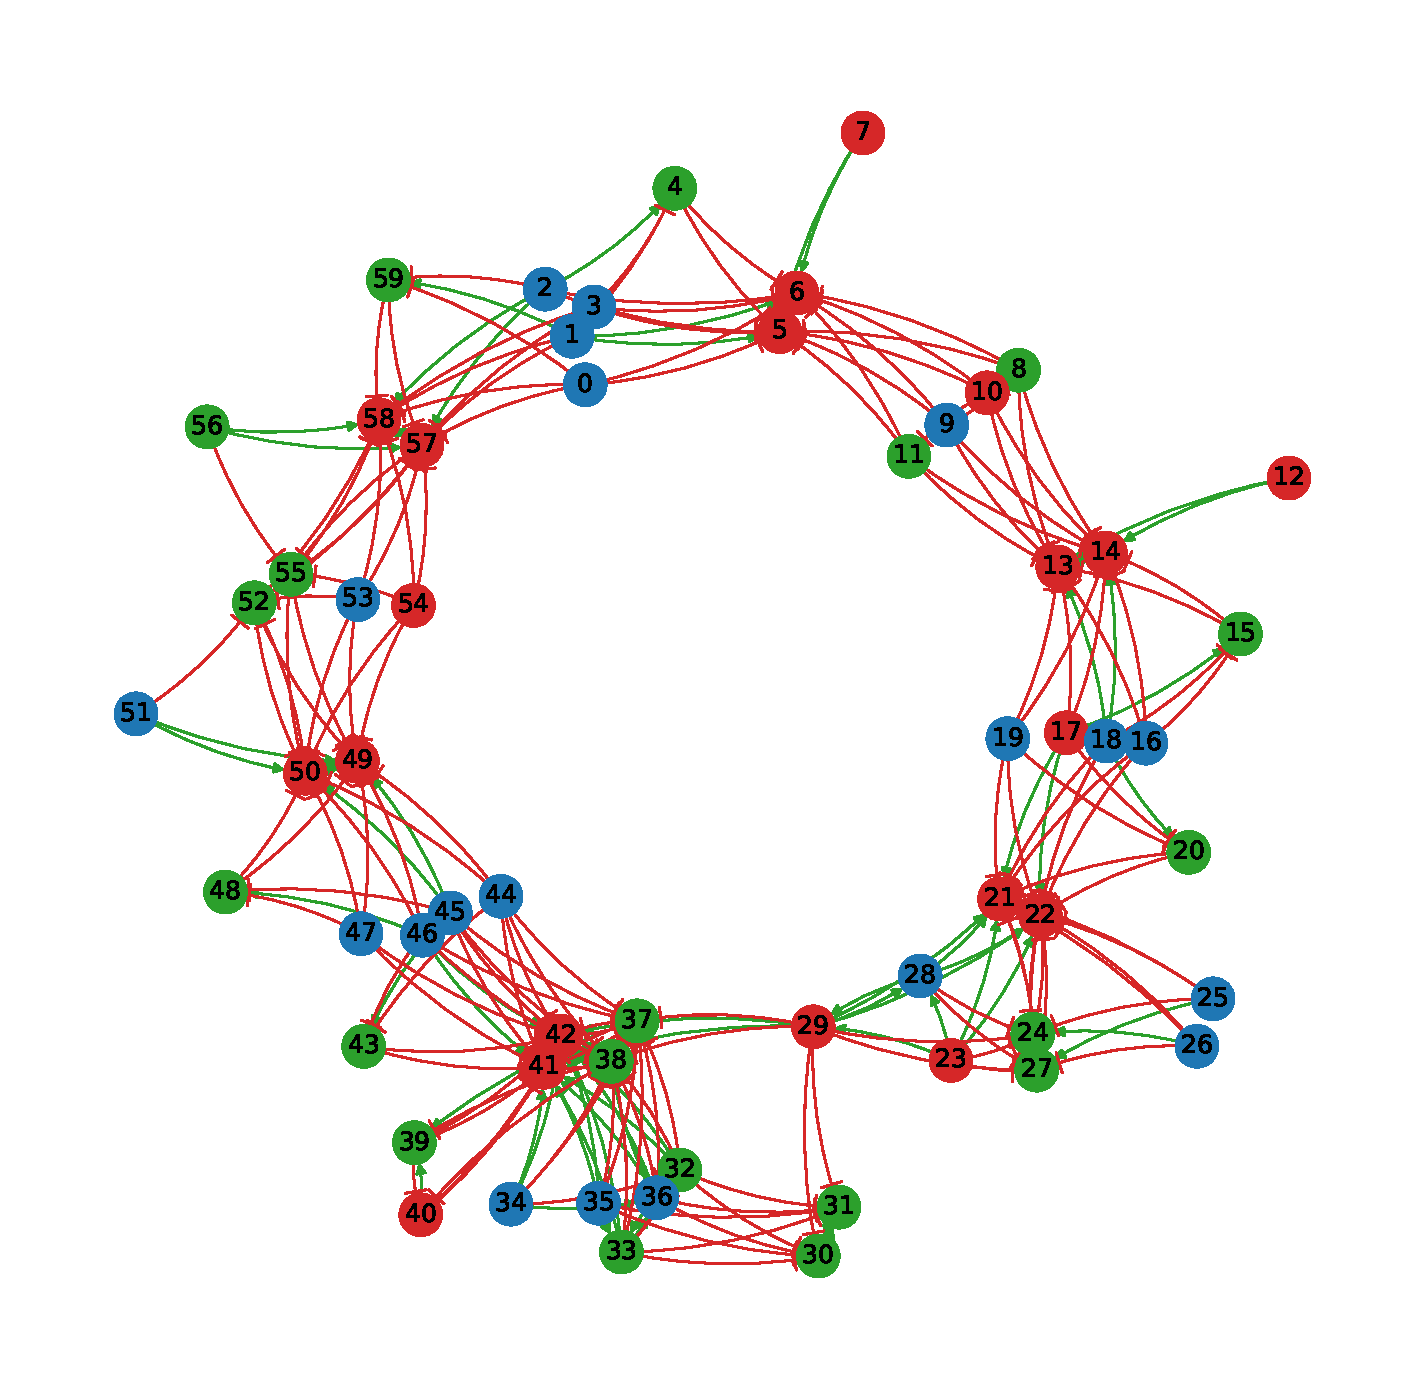
\includegraphics[width=\textwidth]{ploscb/img/combined_effective_graph_rep21_graphviz.pdf}
  \end{subfigure}
  \hspace*{-0.75cm}
  \begin{subfigure}[c]{0.29\textwidth}
    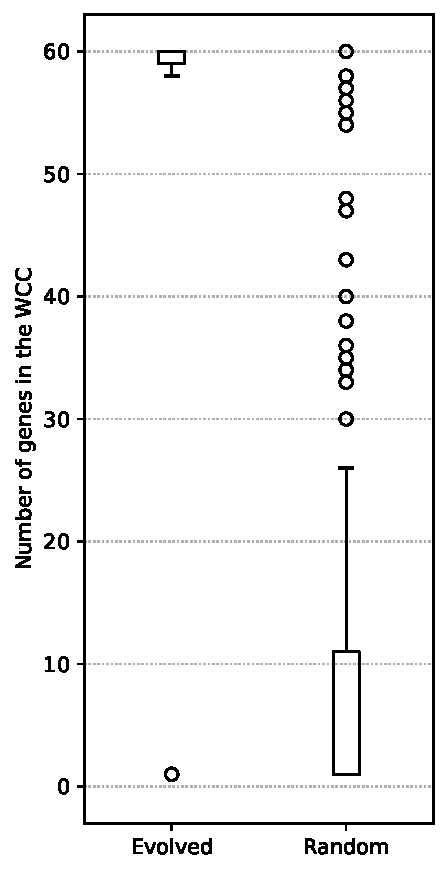
\includegraphics[width=\textwidth]{ploscb/img/effective_graph_wcc_distr.pdf}
  \end{subfigure}
  \caption[Effective interaction graph of an evolved individual, and distribution of effective interaction graph WCCs in evolved and random individuals]{Left: effective interaction graph of the best individual at the last generation of replicate 21, obtained by knocking out each gene and measuring the resulting gene switches in each environment.
  Activation edges are drawn in green, and inhibition edges in red.
  The numbering of the genes is the same as in Figures~\ref{fig:ploscb:genomes},~\ref{fig:ploscb:ko_genomes} and~\ref{fig:ploscb:ko_genomes}.
  Right: distribution of weakly connected component (WCC) sizes in the effective interaction graphs of the evolved individuals (left) and the random individuals (right).}
  \label{fig:ploscb:ko_graph}
\end{figure}

\paragraph{Constructing Effective Interaction Graphs}
In order to construct the effective interaction graph introduced above, we simply add an edge from a gene to every other gene whose activation state is switched by knocking out that gene, in one environment or the other.
If the knockout switches off a gene that was activated in the complete genome, we mark the edge as an activation edge, meaning that the knocked-out gene was necessary to activate the switched gene.
If the knockout switches on a gene that was inhibited in the complete genome, we conversely mark the edge as an inhibition edge.
If knocking out a gene switches the same gene in the two environments, we only add the edge once (we do not build a multigraph).
The effective interaction graph of our example individual is presented on the left-hand side of Figure~\ref{fig:ploscb:ko_graph}.
In the case of this individual, there is a single weakly connected component (WCC), meaning that all genes interact as part of a single whole-genome regulatory network; this is the case in the best individual of 26 out of the 30 replicates.

\paragraph{Structure of the Effective Interaction Graphs}
We computed the effective interaction graph of the best individual in each replicate, and compared these graphs with the effective interaction graphs of 30 random individuals drawn using the same genome parameters (in Table~\ref{tab:param_values}).
The results are presented on the right-hand side of Figure~\ref{fig:ploscb:ko_graph}.
The effective interaction graphs of evolved individuals are clearly different from the interaction graphs of random individuals.
We can see that the evolved genomes have WCC sizes of 58 to 60 genes, comprising nearly every to every gene on the genome, along with very few single-gene WCCs (left).
On the other hand, WCC sizes in the random genomes span the whole range from single-gene to whole-genome WCCs, with most of the connected components counting less than 10 genes (right).

\begin{figure}[H]
  \begin{subfigure}[t]{0.49\textwidth}
    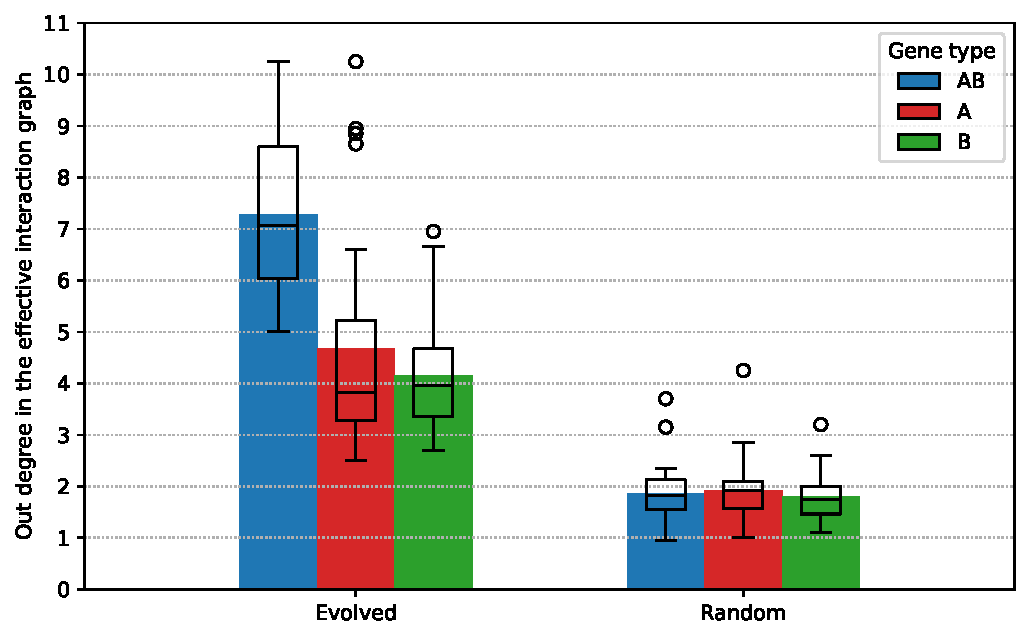
\includegraphics[width=\textwidth]{ploscb/img/effective_graph_combined_out_degree.pdf}
  \end{subfigure}
  \begin{subfigure}[t]{0.49\textwidth}
    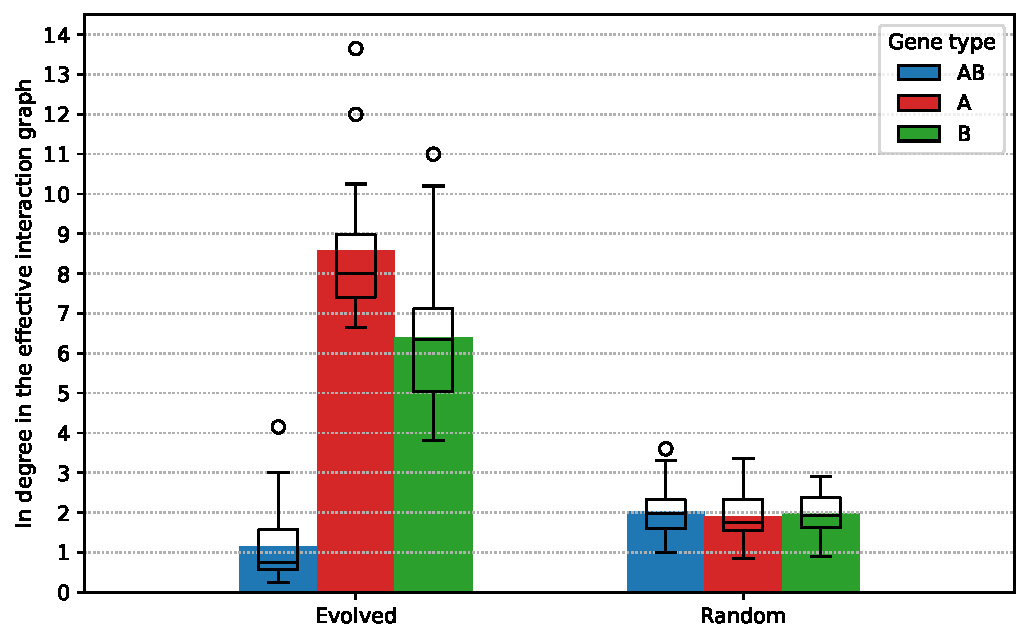
\includegraphics[width=\textwidth]{ploscb/img/effective_graph_combined_in_degree.pdf}
  \end{subfigure}
  \caption[Average in- and out-degree of effective interaction graph nodes for evolved and random individuals]{Left: average out-degree (number of genes switched by knocking out a given gene) of the nodes in the effective interaction graph, separated by gene type, for evolved and random individuals.
  Right: average in-degree (number of genes whose knockout switches a given gene) of the nodes in the effective interaction graph, separated by gene type, for evolved and random individuals.}
  \label{fig:ploscb:ko_data}
\end{figure}

The evolved genomes are indeed much more connected than the random genomes, as we can see in Figure~\ref{fig:ploscb:ko_data}, which presents the out- and in-degree of genes (averaged by gene type) in the effective interaction graphs of the genomes.
The left-hand side of Figure~\ref{fig:ploscb:ko_data} shows the average out-degree of each gene type, or the number of genes that are switched by knocking out a gene of that type.
While knocking out a gene in a random genome switches the state of just under 2 other genes on average, the figure is much higher in the evolved genomes.
Knocking out \emph{A} and \emph{B} genes switches 4 other genes on average, and knocking out \emph{AB} genes up to 7 other genes;
\emph{AB} genes therefore play a quantitatively more important regulatory role than \emph{A} genes or \emph{B} genes, which can be explained by the fact that \emph{AB} genes are activated in both environments, while most \emph{A} and \emph{B} genes are inhibited in one environment or the other.

When looking at the in-degree of the genes, or the number of genes whose knockout will make a given gene switch activation states, we can see that the evolved genomes are again much more connected than the random genomes, and that the in-degree depends on the type of the gene.
Indeed, \emph{AB} genes are only switched by one other gene on average, meaning that their activation state is robust to perturbations in the regulatory network.
The robustness of \emph{AB} gene state is expected, as these genes must have the same activation state in both environments.
On the contrary, \emph{A} genes and \emph{B} genes have an in-degree that is much higher, meaning that their activation state relies on the regulatory action of a large number of other genes, making them more sensitive to the variations between the two environments.

The evolution of the the relative positions of genes on the genome, by leveraging the feedback loop between the transcription of neighboring genes that is mediated by DNA supercoiling, therefore results in our model in the emergence of gene regulatory networks that connect the whole genome into a single entity, rather than a juxtaposition of independent subnetworks.
The network structure that evolves furthermore allows genes to dampen, or amplify, the result of the environmental shift in supercoiling on their activation states, as required by their evolutionary targets.

\section{Discussion and Perspectives}

DNA supercoiling, through its effect on promoter activation~\citep{forquet2021}, is an important actor of the regulatory response of bacteria to changing environmental conditions~\citep{martisb.2019}.
But supercoiling itself is in return impacted by transcription, as presented in the twin-domain model of~\cite{liu1987}.
Indeed, transcription has been shown to play a major role in shaping the bacterial DNA supercoiling landscape~\citep{visser2022}.
Taken together, these observations raise the question of the extent to which the position itself of genes on the genome can regulate their activity, via the coupling of the transcription levels of neighboring genes through local changes in DNA supercoiling.

In order to assess the theoretical possibility of the evolution of such a gene regulatory network, and to determine the potential consequences of the evolution of such a network on the organization of the genome, we developed in this work an evolutionary model of the transcription-supercoiling coupling (expanding upon a proof-of-concept presented in~\cite{grohens2021}), in which populations of individuals must evolve differentiated gene expression levels in response to different environmental conditions, with the transcription-supercoiling coupling as the only regulatory mechanism and inversions as the only mutational operator.
As a the dynamic supercoiling level between actively transcribed genes would be very difficult to model quantitatively, our model voluntarily stays very simple in this regard, and focuses instead on providing a qualitative overview of the range and complexity of the regulatory interactions between neighboring genes that can be mediated by the transcription-supercoiling coupling.

We showed that, in this model, gene regulation by DNA supercoiling is indeed a sufficient mechanism to evolve environment- and gene-specific patterns of activation and inhibition.
In particular, we observed the emergence of genes that are more expressed in a relaxation-inducing environment (or relaxation-activated genes), even though this behavior goes against the facilitated opening of the -10 promoter element by RNA polymerase during the initiation of transcription~\citep{forquet2021}.
%, and is accordingly quite unfrequent in \emph{in vitro} transcription data (where isolated promoters are expressed on plasmids).
This property has been analyzed in detail \emph{in vivo} in the classical example of the \emph{gyrA} promoter, and was shown to result from the unusual sequence of that promoter~\citep{menzel1987}, but for many other genes, this property is less firmly established and depends on the experimental conditions, with experiments finding a proportion of relaxation-activated genes varying between 27\% and 70\% in \emph{S. enterica}~\citep{pineau2022a}.
Our results demonstrate that this behavior can result not only from the specific sequence of the promoter (as for the \emph{gyrA} promoter), but also from the local genomic organization (as suggested in~\cite{elhoudaigui2019}), and confirm the importance of this additional mode of regulation for the first time in an evolutionary simulation.
%A global relaxation of DNA can indeed result in the local hypercoiling, and hence high expression, of genes that happen to be located in the right genetic context.
%The regulation of gene expression by local changes in DNA supercoiling therefore provides a possible causal mechanism for the activity of the relaxation-activated genes found in \emph{E. coli}~\citep{peter2004,sobetzko2016}, \emph{S. enterica}~\citep{webber2013}, or \emph{D. dadantii}~\citep{pineau2022}.

We found that evolved genomes in the model are enriched in divergent pairs of always-active genes, as well as in convergent pairs that act as bistable toggle switches~\citep{gardner2000,johnstone2022}; the evolution of such systems substantiates the theoretical predictions made by models that explicitly describe the movement of RNA polymerases during gene transcription, such as~\cite{sevier2021}.
Then, we showed that the local organization of the genome into convergent or divergent pairs of genes is not sufficient to explain the transcriptional response of individuals to different environments, but that larger subnetworks can be required to selectively inhibit genes in specific environments.
Such regulation of gene expression through interaction with groups of neighboring genes could help explain the evolutionary persistence of synteny groups between \emph{E. coli} and \emph{S. enterica}~\citep{junier2016}, as well as through the evolutionary history of \emph{B. aphidicola}~\citep{brinza2013}.
Indeed, we show that local interactions can play a role in regulating the expression of neighboring genes, and genomic rearrangements might disrupt these local interactions.
Finally, we used transcriptional knockouts, adapting the  classical tool of gene knockouts~\citep{baba2006} to our transcription-centric model, in order to characterize the evolved gene regulatory networks in further detail.
We first showed that these regulatory networks integrate the entire genome of evolved individuals into a single connected unit, in opposition to the sparser, disconnected regulatory networks displayed by randomly generated individuals.
Then, we showed that the structure of these networks leverages the transcription-supercoiling coupling to increase or decrease the sensitivity of genes to perturbations in the regulatory network, strengthening the differentiated expression patterns that are the evolutionary target for each gene type.

All in all, our simulations demonstrate that the transcription-supercoiling coupling provides a regulatory mechanism that is precise enough for the evolution of complex regulation patterns that only depend on the arrangement of genes on the genome.

Several work directions still remain open to investigation.
From an evolutionary perspective, the experimental framework in which we tested our model is at present very simple, and could be extended.
The desired gene expression levels in our model are binary, targeting maximal or minimal transcription, but could be replaced by an arbitrary level between these values for each gene, in order to see whether the local organization into pairs as well as the whole-genome regulatory network that we described are preserved under these less constrained conditions.
Similarly, we could refine the environmental challenge faced by individuals by evaluating them in each environment in succession, rather than separately, or by continuously changing the environment over evolutionary time.
From a theoretical perspective, a range of mechanistic biophysical models of the transcription-supercoiling coupling have been put forward, with different hypotheses underpinning the coupling:~\cite{brackley2016} shows a phase transition in the transcription regime as the number of transcribing RNA polymerases increases;~\cite{sevier2021} shows that bursty transcription can emerge from the transcription-supercoiling coupling; and~\cite{meyer2014} and~\cite{elhoudaigui2019} try to predict gene expression levels quantitatively from the local DNA supercoiling level.
An important vindication of these theoretical approaches to the interplay between supercoiling and transcription would therefore be to verify the extent to which these models, including ours, conform to one another as the level of abstraction changes.
Moreover, integrating a model of gene regulation by DNA supercoiling into a more comprehensive evolutionary model of the genome that allows for classical gene regulation via transcription factors, such as the model presented in~\cite{crombach2008}, would help shed light on the coevolution between the different modes of gene regulation that are available to bacterial genomes.
Finally, from an experimental perspective, a better understanding of the regulatory interactions caused by the transcription-supercoiling coupling could help design more reliable synthetic genetic constructs, as explored in~\cite{johnstone2022}.


\section{Conclusion}

To the best of our knowledge, our work is the first to model the regulatory role of supercoiling on transcription at a many-gene scale, using evolutionary simulations.
It demonstrates the importance of the direct interactions between genes that are mediated by local changes in DNA supercoiling on their transcription rates, as well as the precision and versatility of the regulatory activity stemming from these interactions.
For experimentalists, it provides an underlying theory that could help explain the heterogeneous transcriptomic response (with both up- and down-regulation of multiple genes) observed in bacteria confronted to supercoiling variations, due among others to virulence-inducing environments~\citep{dorman2019} or to gyrase-inhibiting antibiotics~\citep{delacampa2017}.
For evolutionists, it provides a plausible evolutionary rationale for the observed conservation of local gene order between closely related bacteria~\citep{junier2016} and along evolutionary histories~\citep{brinza2013}.
Finally, for synthetic biologists, it provides a theory to help predict in finer detail the gene transcription levels that can be expected from a given gene syntax~\citep{johnstone2022}, which could help design more robust genetic circuits.
